\documentclass[12pt]{article}
\usepackage[a4paper, total={6.5in, 10in}]{geometry}
\PassOptionsToPackage{quiet}{fontspec}
\usepackage{ctex}
\usepackage{float}
\usepackage{tikz, pgfplots}
\usepackage{2d_plot/2d_plot}
\pgfplotsset{compat=1.18}
\usetikzlibrary{arrows.meta}
\usetikzlibrary{intersections}
\usetikzlibrary{patterns}
\usetikzlibrary{positioning}


% code print environment
\usepackage{listings}
\lstset{
    aboveskip=3mm,
    belowskip=3mm,
    showstringspaces=false,
    columns=flexible,
    rulecolor=\color{gray},
    backgroundcolor=\color{white},
    numbers=left,
    numbersep=5pt,
    numberstyle=\fontsize{8pt}{8pt}\selectfont\color{gray}\ttfamily,
    breaklines=true,
    postbreak=\raisebox{0ex}[0ex][0ex]{\ensuremath{\hookrightarrow\space}},
    breakatwhitespace=true,
    tabsize=4,
}
\lstnewenvironment{codeprint}[1][10]           % setting default code fontsize = \normalsize 
{
    \lstset{%
        frame=tlb,
        frameround=fftt,
        aboveskip=1em,
        basicstyle=\fontsize{#1pt}{#1pt}\selectfont\ttfamily,
    }
}{}

\title{TikZ 坐标系统}
\author{Eureka}
\date{\today}


% \newcommand{\ddt}[2][]{\fill[#1] (#2) circle(1pt);}
\newcommand{\lrl}{~\ensuremath{\Longleftrightarrow}~}


\begin{document}
\maketitle
\tableofcontents
\clearpage


\section{基础知识}
常用的\verb|\draw,\fill,\shade|和\verb|\filldraw|命令,实际上
都是带某些选项的\verb|\path|命令的简写,详情可以参见pgfmanual的p172的\verb|actions on paths|内容.
\begin{itemize}
    \item \verb|\draw| \lrl\verb|\path[draw]|
    \item \verb|\fill| \lrl\verb|\path[fill]|
    \item \verb|\clip| \lrl\verb|\path[clip]|
    \item \verb|\shade| \lrl\verb|\path[shade]|
    \item \verb|\filldraw| \lrl\verb|\path[fill, draw]|
    \item \verb|\node| \lrl \verb|\path node|
\end{itemize}


\subsection{draw命令}
\begin{itemize}
    \item \textbf{tikz中坐标系的默认单位,通常是cm; 但是在scope中指定偏移时一定要带上cm单位,默认单位不对}
    \item 相对坐标: \verb|+, ++|的区别, \verb|+|始终以第一个点为偏移参考点,这里每次的便宜参考点均为 $(0, 1)$;但是
        在\verb|++|中,第二次的参考点即为 $(0, 1)+(1, -1)$. 以下分别为两幅图的代码:
        \begin{verbatim}
            \draw (0,1) -- +(1,-1) -- +(1,1);
            \draw (0,1) -- ++(1,-1) -- +(1,1);
        \end{verbatim}
        \begin{center}
            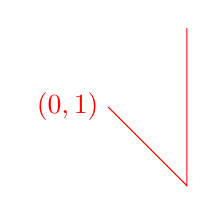
\begin{tikzpicture}
                \draw[red] (0,1)node[left]{$(0, 1)$} -- +(1,-1) -- +(1,1);
                \ShowPoint[color=red] {(0, 1)}
            \end{tikzpicture}
            \hspace*{8em}
            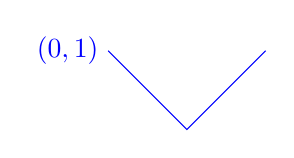
\begin{tikzpicture}
                \draw[blue] (0,1)node[left]{$(0, 1)$} -- ++(1,-1) -- +(1,1);
                \ShowPoint[color=blue] {(0, 1)}
            \end{tikzpicture}
        \end{center}
    \item 极坐标: \verb|(angle:distance)|
    \item 坐标运算:需要导入\verb|calu|库: \verb|\usetikzlibrary{calc}|,使用格式为:\par
        \verb|\draw (0,1) -- ($(0,1)-2*(-1,1)$);|
    \item draw命令的复用:在一个\verb|\draw|中可以同时绘制多条线段,用法如下\par
        \verb|\draw (0,0) -- (1,1) (0,1) -- (1,0);|
    \item draw绘制闭合曲线:一定要加上 \verb|-- cycle;| 
    \item 绘制过两点的直角折线: \verb!\draw (0,0) |- (1,1);! 与 \verb!\draw (0,0) -| (1,1);!
        \begin{center}
            \begin{tikzpicture}
                \draw (0,0)node[left]{$(0, 0)$} |- (1,1)node[right]{$(1, 1)$};
                \ShowPoint[color=gray] {(0, 0); (1, 1)}
            \end{tikzpicture}
            \hspace*{8em}
            \begin{tikzpicture}
                \draw (0,0)node[left]{$(0, 0)$} -| (1,1)node[right]{$(1, 1)$};
                \ShowPoint[color=gray] {(0, 0); (1, 1)}
            \end{tikzpicture}
        \end{center}
    \item 网格线绘制: \verb|\draw[step=0.5] (0,0) grid (3,2);|x
    \item draw绘制描点折线: \verb|\draw plot coordinates {(0,0) (1,2) (2,1) (4,2)};|
\end{itemize}


\subsection{node 命令}
\begin{itemize}
    \item node 形状: \verb|\node[shape=rectangle]|
    \item node 填充: \verb|\node[fill=red]|, 预先定义好的节点形状有三种:矩形(rectangle), 圆形(circle), 和点形(coordinate)
    \item node 描边: \verb|\node[draw=red]|, 默认不描边,使用draw=none可以取消描边
    \item node 文本: \verb|\node[text=red]|
    \item node 的anchor:默认为文本中心.% 
        
\begin{tikzpicture}
            \draw[fill=blue, draw=none] (0,0) circle (2pt);
            \node[anchor=center] at (0,0) {CENTER};
        \end{tikzpicture}
    \item node 文本位置: 需\verb|positioning|库,语法:\verb|\node[below right=8mm and 4mm] ...;|
    \item node 连接点设置: 给定节点名称\verb|\node (a) at (x, y) {};|之后,\par 
        \verb|a.east, a.west, a.south, a.north, a.south|\par
        \verb|east, a.south west, a.north east, a.north west|
        均可使用.
    \item coordinate:和node的突然标注类似,我们也可以使用coordinate进行临时标记,语法如下:
        \verb|\draw (1, 1)node[]{} -- (2, 2)coordinate(c);|
        然后我们在之后便可以使用\verb|(c)|这个点,甚至可以这样:\par
        \verb|\draw (1, 1) -- (2, 2)coordinate(c)node[left]{node $c$};|
\end{itemize}


\subsection{Curvels}
\begin{itemize}
    \item arc:arc命令有时是极为方便的,基本的参数中
    \item Bessel curvel\par 
        此时需要将\verb|\draw|中的\verb|--|操作改为\verb|..|操作, 添加曲线切线公共点,
        即\verb|control|命令,于是完整的命令为:
        \begin{verbatim}
            \draw (0,0) .. controls (1,1) .. (4,0);
        \end{verbatim}
        \begin{center}
            \begin{tikzpicture}
                \draw[blue] (0,0) .. controls (1,1) .. (4,0);
                \ShowPoint[color=red] {(1, 1)}
            \end{tikzpicture}
        \end{center}

        \begin{verbatim}
            \draw (0,0) .. controls (1,1) and (2,1) .. (4,0);
        \end{verbatim}
        \begin{center}
            \begin{tikzpicture}
                \draw[blue] (0,0) .. controls (1,1) and (2,1) .. (4,0);
                \ShowPoint[color=red] {(1, 1); (2, 1)}
            \end{tikzpicture}
        \end{center}

    \item in 和 out \par  
        使用另外一种方式,使用 \verb|in, out|两参数设置初值和结束角度:
        \begin{verbatim}
            \draw[green] (-6, -4) to[out=60, in=-120] (-2, -4);
        \end{verbatim}
        \begin{center}
            \begin{tikzpicture}
                \draw[green] (-2, 0) to[out=60, in=-120] (2, 0);
                \draw (-3, 0) -- (3, 0);
                \draw[dashed] (-2, 0) -- +(60:.5) -- +(-120:.5);
                \draw[dashed] (2, 0) -- +(60:.5) -- +(-120:.5);
                \ShowPoint[color=red] {(-2, 0); (2, 0)}
            \end{tikzpicture}
        \end{center}
    \item 描点曲线\par 
        给 plot 操作加上 smooth 选项将用光滑曲线连接各点.而 tension
        选项描述该光滑曲线的绷紧度,取值范围为从 0 到 1,默认值为 0.55.\par 
        \verb|\draw[color=red] plot[smooth, tension=.9] coordinates ...;|
        \begin{center}
            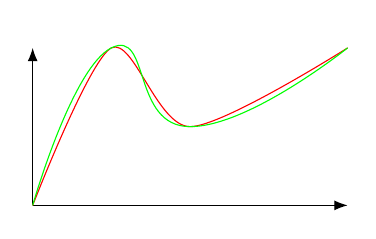
\begin{tikzpicture}[>=Latex]
                \draw[->] (0,0) -- (4,0);
                \draw[->] (0,0) -- (0,2);
                \draw[color=red] plot[smooth] coordinates {(0,0) (1,2) (2,1) (4,2)};
                \draw[color=green] plot[smooth, tension=.9] coordinates {(0,0) (1,2) (2,1) (4,2)};
                \ShowPoint[color=blue] {(0, 0); (1, 2); (2, 1); (4, 2)}
            \end{tikzpicture}
        \end{center}
    \item smooth cycle\par 
        如果将选项 smooth 改为 smooth cycle,将绘制一条闭合曲线.\par 
\begin{codeprint}
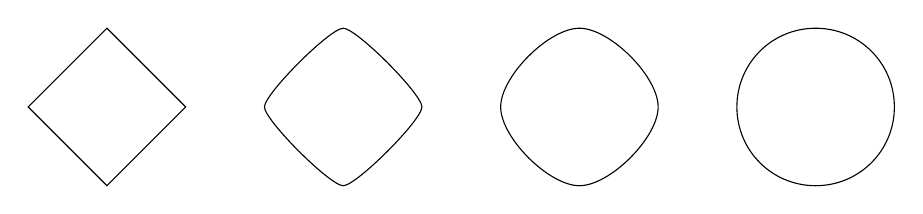
\begin{tikzpicture}[smooth cycle]
    \draw plot[tension=0] 
        coordinates {(0,1) (1,0) (2,1) (1,2)};
    \draw[xshift=3cm] plot[tension=0.3]
        coordinates{(0,1) (1,0) (2,1) (1,2)};
    \draw[xshift=6cm] plot[tension=0.7]
        coordinates{(0,1) (1,0) (2,1) (1,2)};
    \draw[xshift=9cm] plot[tension=1]
        coordinates{(0,1) (1,0) (2,1) (1,2)};
\end{tikzpicture}
\end{codeprint}
        \begin{center}
            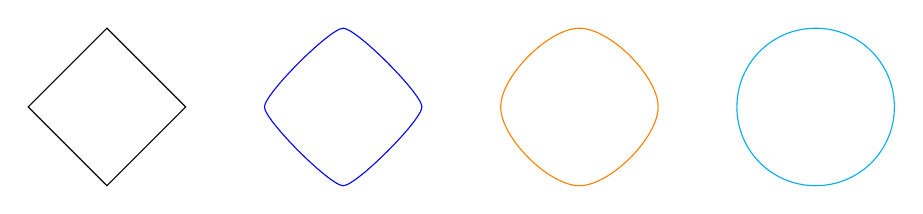
\begin{tikzpicture}[smooth cycle]
                \draw plot[tension=0, draw=red] 
                    coordinates {(0,1) (1,0) (2,1) (1,2)};
                \draw[xshift=3cm, draw=blue] plot[tension=0.3]
                    coordinates{(0,1) (1,0) (2,1) (1,2)};
                \draw[xshift=6cm, draw=orange] plot[tension=0.7]
                    coordinates{(0,1) (1,0) (2,1) (1,2)};
                \draw[xshift=9cm, draw=cyan] plot[tension=1]
                    coordinates{(0,1) (1,0) (2,1) (1,2)};
            \end{tikzpicture}
        \end{center}
\end{itemize}

\subsection{positioning库}
\begin{itemize}
    \item node文本同时指定多方向偏移量: \verb|\node[below right=8mm and 4mm] ...;|
    \item node文本偏移量可为数学表达式: \verb|\node[below=8mm/2+4pt*2] ...;|
    \item node节点之间的相对位置:\verb|\node[fill=gray,right=1cm of a] (b) {B};|
\end{itemize}




\subsection{路径交点}
此时你需要使用intersections库, \verb|\usetikzlibrary{intersections}|,使用语法为:
\begin{codeprint}
% Name the coordinates, but do not draw anything:
\path [name intersections={of=<path 1> and <path 2>}];
\coordinate (C) at (intersection-1);
\end{codeprint}

\begin{itemize}
    \item 示例 1:在循环中使用
\begin{codeprint}
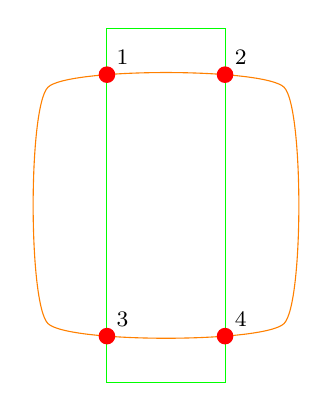
\begin{tikzpicture}[
        every node/.style={black,above right}, 
        smooth cycle, scale=3
    ]
    \draw[draw=orange, name path=line 1] plot[tension=0.3]
        coordinates{(0, 0) (0,1) (1,1) (1,0)};
    \draw[draw=green, name path=line 2] 
        (.25, -.25) rectangle (.75,1.25);
    \fill[red,name intersections={of=line 1 and line 2,total=\t}]
        \foreach \s in {1,...,\t}
            {(intersection-\s) circle (1pt) node {\footnotesize\s}};
\end{tikzpicture}
\end{codeprint}
    \begin{center}
        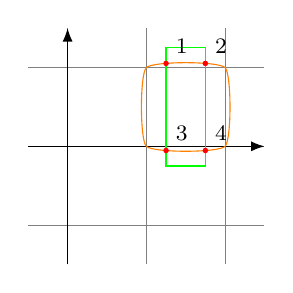
\begin{tikzpicture}[every node/.style={black,above right}, smooth cycle, >=Latex]
            % coordinate
            \draw[help lines] (-1.5, -1.5) grid (1.5, 1.5);
            \draw[->] (-1.5, 0) -- (1.5, 0);
            \draw[->] (-1, -1.5) -- (-1, 1.5);
            \begin{scope}[scale=1]
                % two paths
                \draw[draw=orange, name path=line 1] plot[tension=0.3]
                    coordinates{(0, 0) (0,1) (1,1) (1,0)};
                \draw[draw=green, name path=line 2] (.25, -.25) rectangle (.75,1.25);
                \fill[red,name intersections={of=line 1 and line 2,total=\t}]
                    \foreach \s in {1,...,\t}{(intersection-\s) circle (1pt) node {\footnotesize\s}};
            \end{scope}

        \end{tikzpicture}
    \end{center}


    \item 示例 2:不显式调用(不用设置变量来接受返回值),使用\verb|intersection-<num>|
        表示第\verb|<num>|个交点.
\begin{codeprint}
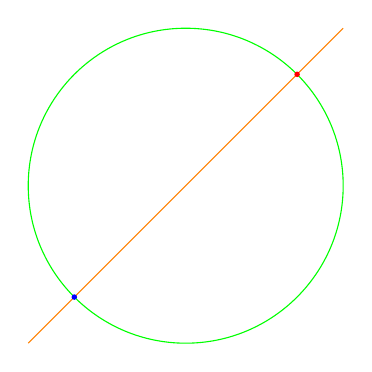
\begin{tikzpicture}
    \draw[orange, name path=line 1] (-2, -2) -- (2, 2);
    \draw[green, name path=circle 1] (0, 0) circle (2);
    % get the intersections(by don't get it by return value)
    \path[name intersections={of=line 1 and circle 1}];
    \fill[red] (intersection-1) circle (1pt); 
    \fill[blue] (intersection-2) circle (1pt); 
\end{tikzpicture}
\end{codeprint}
    \begin{center}
        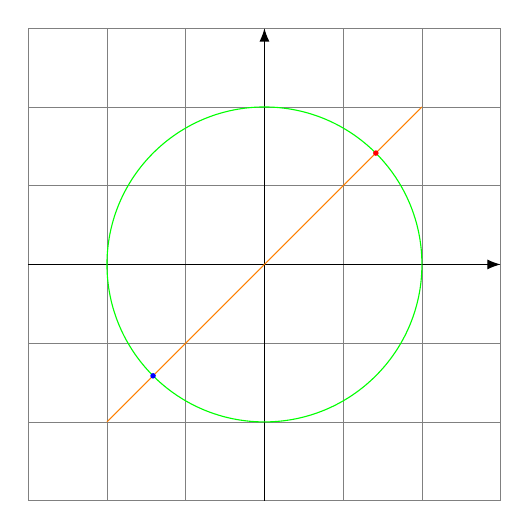
\begin{tikzpicture}[>=Latex]
            % coordinate
            \draw[help lines] (-3, -3) grid (3, 3);
            \draw[->] (-3, 0) -- (3, 0);
            \draw[->] (0, -3) -- (0, 3);
            % two paths
            \draw[orange, name path=line 1] (-2, -2) -- (2, 2);
            \draw[green, name path=circle 1] (0, 0) circle (2);
            % get the intersections(by don't get it by return value)
            \path[name intersections={of=line 1 and circle 1}];
            \fill[red] (intersection-1) circle (1pt); 
            \fill[blue] (intersection-2) circle (1pt); 
        \end{tikzpicture}
    \end{center}
    \item 示例 3:不同scope之间共享, 此时需要把原始的 \par  
        \verb|name path=<path name>| $\longrightarrow$ \verb|name path global=<path name>|,
        下面及一个最小示例:
\begin{codeprint}
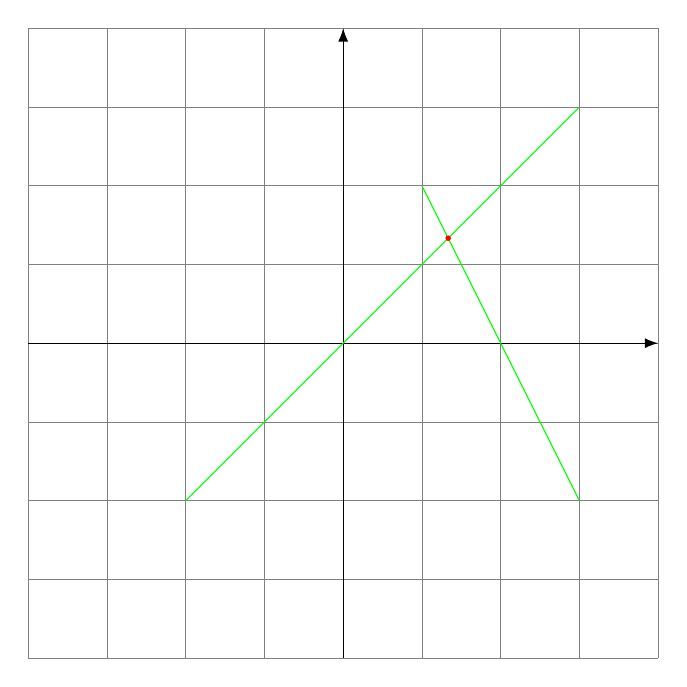
\begin{tikzpicture}[>=Latex]
    \draw[help lines] (-4, -4) grid (4, 4);
    \draw[->] (-4, 0) -- (4, 0);
    \draw[->] (0, -4) -- (0, 4);
    \begin{scope}
        \draw[green, name path global=line 1] (-2, -2) -- (3, 3);
    \end{scope}
    \begin{scope}[xshift=2cm]
        \draw[green, name path global=line 2] (-1, 2) -- (1, -2);
    \end{scope}
    % out of scope to get the intersections
    \path[name intersections={of=line 1 and line 2}];
    \fill[red] (intersection-1) circle (1pt);
\end{tikzpicture}
\end{codeprint}
        \begin{center}
            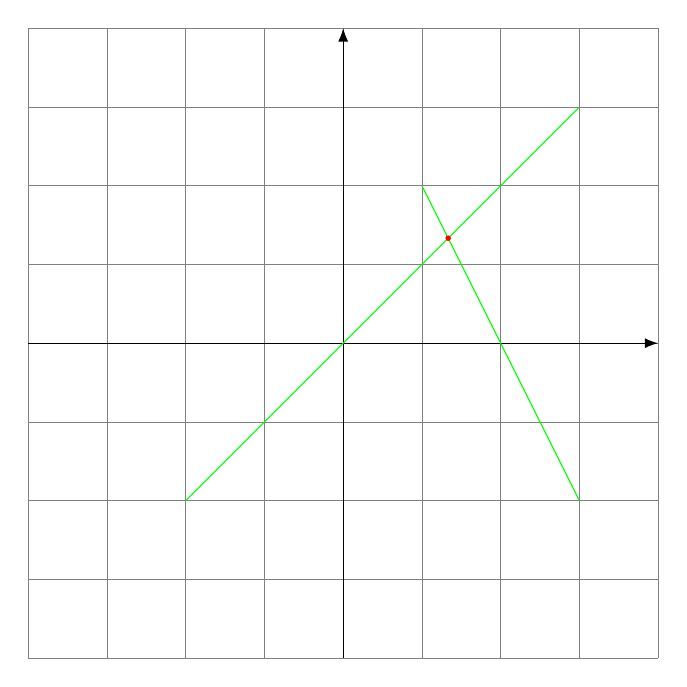
\begin{tikzpicture}[>=Latex]
                \draw[help lines] (-4, -4) grid (4, 4);
                \draw[->] (-4, 0) -- (4, 0);
                \draw[->] (0, -4) -- (0, 4);
                \begin{scope}
                    \draw[green, name path global=line 1] (-2, -2) -- (3, 3);
                \end{scope}
                \begin{scope}[xshift=2cm]
                    \draw[green, name path global=line 2] (-1, 2) -- (1, -2);
                \end{scope}
                % out of scope to get the intersections
                \path[name intersections={of=line 1 and line 2}];
                \fill[red] (intersection-1) circle (1pt);
            \end{tikzpicture}
        \end{center}
\end{itemize}


\subsection{路径剪裁}
对于要使用填充功能的用户来说,路径剪裁是必须知道的,最起码得知道
\verb|\clip|命令。不要认为这个命令很复杂,实际上你把这个clip裁剪的区域
看作\textbf{定义域}即可,之后所有的绘图,或者是填充均只会出现在定义域,也即clip区域,
也就是和clip做交集得到的区域.



\clearpage
\subsection{支持函数}
这里有一个关于函数写法注意事项:
\textbf{只要你的函数表达式含有(),那么你的怎么函数表达式就需要使用}\verb|{}|\textbf{来包围.}

比如下面的正确示例:
\begin{codeprint}
\draw[smooth, purple, domain=-6.927:6.927] plot (\x, {sqrt(16 - pow(\x, 2)/3)});
\end{codeprint}

加入你写作下面这样就是错误的:
\begin{codeprint}
\draw[smooth, purple, domain=-6.927:6.927] plot (\x, sqrt(16 - pow(\x, 2)/3));
\end{codeprint}

PGF(TiKZ) 的数学引擎支持下面这些数学函数:
\begin{center}
    \begin{tabular}{ccccc}
        \hline
        abs & cot & hex & neg & rnd \\
        acos & deg & Hex & not & round \\
        add & depth & int & notequal & sec \\
        and & div & ifthenelse & notgreater & sin \\
        array & divide & less & notless & sinh \\
        asin & e & ln & oct & sqrt \\
        atan & equal & log10 & or & subtract \\
        atan2 & factorial & log2 & pi & tan \\
        bin & false & max & pow & tanh \\
        ceil & floor & min & rad & true \\
        cos & frac & mod & rand & veclen \\
        cosec & greater & Mod & random & width \\
        cosh & height & multiply & real & \\
        \hline
    \end{tabular}            
\end{center}



\clearpage
\section{绘图库\texttt{2d\_plot}}
\subsection{基础命令}
这里主要是依靠Geogebra来估计交点的坐标,当然前面已经提到,我们可以使用自带的intersection库进行交点的求解.
本库的基本命令有以下函数提供:
\begin{itemize}
    \item \verb|\NormalPlot|
    \item \verb|\ParamPlot|
    \item \verb|\ShowPoint|
    \item \verb|\ShowIntersections|
    \item \verb|\ShowGrid|
    \item \verb|\NormalPlotPrecise|
    \item \verb|\ParamPlotPrecise|
\end{itemize}

由于pgfplots包太过于底层,且个人感觉没有tikz方便,于是本人没有对pgfplots宏包下
太大的功夫.

\subsection{函数绘制}
同时这里为了解决tikz自身的计算能力不足问题,我自定义了两个命令:
\begin{codeprint}
\NormalPlot[<\draw cmd's option>][<variable x's domain>]{<2d function>}
\ParamPlot[<\draw cmd's option>][<param t's domain>]{<2d param function>}
\end{codeprint}


\subsection{阴影描绘}
同样的也是基于上面的两个命令\verb|\NormalPlot, \ParamPlot|进行阴影的绘制。此时我们有了两个新的命令
\begin{verbatim}
    \NormalFill[<fill option>][<x domain>] {a set of function}
    \ParamFill[<fill option>][<t domain>] {a set of param function}
\end{verbatim}


\subsection{绘制精度}
并且有如下的备用选项命令\verb|\ParamPlotPrecise|, \verb|\NormalPlotPrecise|, 用于设置
绘图的采样精度,默认在给定区间内平均采样1000个点,可以使用如下命令进行这个参数的更改
\begin{codeprint}
\NormalPlotPrecise{10}  % 更改NarmalPlot采样精度为10个点
\ParamPlotPrecise{10}   % 更改ParamlPlot采样精度为10个点
\end{codeprint}

注意:改变精度命令仅对当前绘图函数的紧邻的第一个绘图命令有影响,不会影响之后的所有绘图命令的
采样精度。如果想要更改之后所有绘图的采样率可以设置默认的影响范围参数\verb|once|为\verb|after|.
但是目前的话,只要你可选参数填的不是once,那么它都是会改变之后的所有采样精度的.
两命令并没有用到pgfplots宏包\verb|axis|环境.


\subsection{点的标注}
使用自定义的\verb|2d_plot|库,可以避免自己进行如下的繁杂代码书写:
\begin{codeprint}
% 1.original plot method for parametric function
\draw[smooth, purple, domain=-6.927:6.927] plot (\x, {sqrt(16 - pow(\x, 2)/3)});
\draw[smooth, purple, domain=-6.927:6.927] plot (\x, -{sqrt(16 - pow(\x, 2)/3)});

% 2.use gnuplot gnerate data
\draw plot[smooth] file {./data.table};
\draw[red] plot[smooth] file {./param_data.table};

% 3.use pgfplots --> ticks is not the same
\begin{axis}               
    \addplot gnuplot[domain=-6:6] {-sqrt(16 - x^2/3)};                
\end{axis} 
\end{codeprint}

同时本绘图库还包含了基本的点的标注功能函数\verb|\ShowPoint|,使用参数如下:
\begin{codeprint}
    \ShowPoint[radius=3pt, color=blue, opacity=.5, style=circle] 
        {(1, 1); (2, 2)}[text1; text2; text3][above left];
\end{codeprint}

其中的每一个点的标注文本\verb|text_i|是可以省略或者是多于欲标注的点的个数的。最后的 
\verb|<style>|选项为标注文本的位置,任意的合法的\verb|\node[<option>]|中的\verb|option|
均可,比如\verb|[above right, font=\small]|

\subsection{交点求解}
本绘图库包含图像(\texttt{path})的交点求解命令\verb|\ShowIntersections|,用于 
绘制两条 \texttt{path}的交点, 使用方法如下:
\begin{codeprint}
    \ShowIntersecions{<path 1 name>; <path 2 name>}{<num of intersections>}
\end{codeprint}

但是目前还不推荐使用此命令,因随之而来的就是使用自定义命令绘制的
path进行交点的求解时可能需要处理的数据过多,导致运行速度变慢.
解决方法如下,同样是使用在线网站Geobebra进行交点坐标的估计.后续也许会考虑使用gnuplot进行
交点的计算,然后返回进行标记.


\subsection{坐标系统绘制}
最后便是一些关于坐标轴的基本设置函数
\begin{itemize}
    \item \verb|\ShowAxis|:即展示坐标轴,调用格式如下:\par
        \verb|\ShowAxis[<axis style>]{<start>; <end>}|
    \item \verb|\ShowGrid|:即展示坐标网格,调用格式如下:\par
        \verb|\ShowGrid[<axis style>]{<start>; <end>}|
\end{itemize}

其上的所有的\verb|<start>|,或\verb|<end>|均为坐标点,格式为\verb|(coor1, coor2)|.

上面的所有\verb|<style>|均为\verb|\draw[<option>]|中的合法\verb|<option>|字典值,
如 \verb|color=red|.


\subsection{绘图示例}
首先是展示使用在线网站Geogebra绘制的示例,同时也是为了展示我们的绘制精准度.
\begin{figure}[!htb]
    \centering
    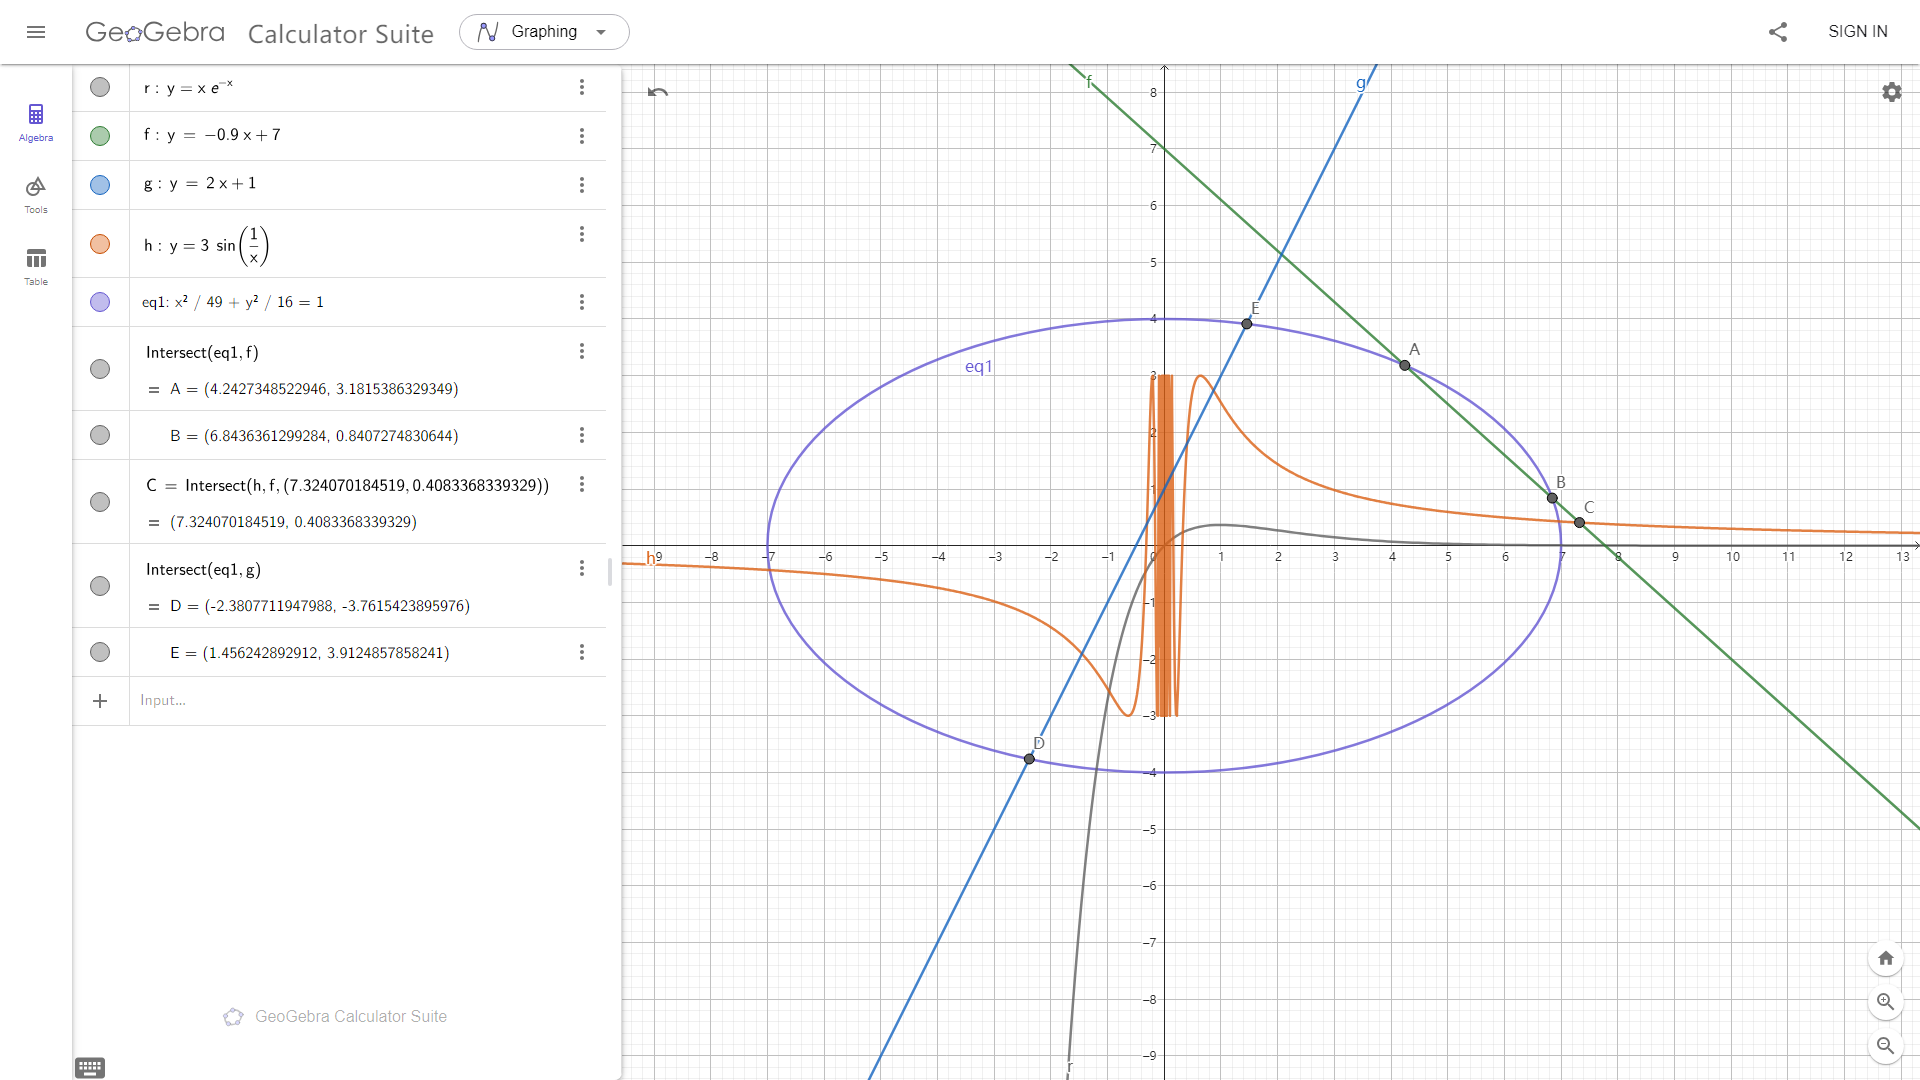
\includegraphics[width=.95\linewidth]{./shoots.png}
\end{figure}


然后下面便是我们使用\texttt{2d\_plot}绘图库的绘制效果,经过这一点其实可以看出
本绘图库的精度是可以非常高的,取决于你设置的gnuplot采样精度.另外,如果不想要使用
本库提供的\verb|\ShowIntersections|命令显示路径交点,那么你可以使用Geogabra绘制完成
之后手动输入交点坐标进行绘制,因本绘图库的坐标和Geogebra的坐标是 $1-1$的.

\begin{figure}[H]
    % \usetikzlibrary{arrows.meta}
    \begin{tikzpicture}[font=\small, >=Latex]
        % draw grid(coordinates)
        % \draw[very thin,color=gray] (-8,-8)node[right]{$(-8, -8)$} grid (8,8)node[left]{$(8, 8)$};
        \ShowGrid{(-8, -8); (8, 8)}
        % \fill[black] (0, 0)node[below]{$O$=(0, 0)} circle (1pt);
        \ShowPoint{(0, 0)}[$O=(0, 0)$][below right=.5em and 1em]
        \ShowAxis {(0, -8); (0, 8)}
        \ShowAxis {(-8, 0); (8, 0)}

        % Test unit
        \fill[red] (-4cm, 4em)node[left]{$A_1$=(-4cm, 4em)} circle (1pt);
        \fill[blue] (-4cm, 4cm)node[left]{$A_2$=(-4cm, 4cm)} circle (1pt);

        % draw function
        \draw[color=orange, domain=-3:3] plot (\x, 2*\x+1);
        \draw[color=cyan, domain=-1:7.6] plot (\x, -.9*\x+7);

        % draw an ellipse
        % 1.use self define cmd
        \NormalPlotPrecise{1500}
        \NormalPlot[][-7:7.8]{3*sin(1/x)}
        \NormalPlot[green, name path=exp][-1.5:7.5] {x*exp(-x)}
        \ParamPlot[red, name path=ellipse][0:2*pi]{7*sin(t), 4*cos(t)}

        % fill(needs \usetikzlibrary{patterns})
        \begin{scope}
            \clip (2, 0) rectangle (8, 1); 
            \fill[pattern=north east lines] plot file{./2d_plot/gnuplot_output_data/data_gen_2.table};
        \end{scope}
        \begin{scope}
            \clip (-6, 0) rectangle (-2, -2);
            \NormalPlot[][-6:-1]{3*sin(1/x)}
            \fill[pattern=crosshatch, pattern color=orange] plot file{./2d_plot/gnuplot_output_data/data_gen_4.table} -- (-2, 0) -- (-6, 0);
        \end{scope}

        % find intersection
        % \ShowIntersecions{exp; ellipse}{2}
        % 或者是如下的语句
        % \path[name intersections={of=exp and ellipse}];
        % \ShowPoint[color=red] {(intersection-1); (intersection-2)}

        % draw intersection dot 
        % annotation can be more than number of points
        \ShowPoint {(2.068, 5.137); (4.242, 3.181); (6.843, 0.840); (7.324, 0.408)}
            [$p_1$; $p_2$; $p_3$; $p_4$; $p_5$; $p_6$; $p_7$][above]
        \ShowPoint[radius=3pt, color=blue, opacity=.5] {(-2.380, -3.761)}
        \ShowPoint[color=orange, opacity=1, radius=2pt] {(1.456, 3.912)}
    \end{tikzpicture}
    \caption{\texttt{2d\_plot}绘制示例}
\end{figure}

绘图示例的代码如下:
\begin{codeprint}
\begin{tikzpicture}[font=\small, >=Latex]
    % draw grid(coordinates)
    \ShowGrid{(-8, -8); (8, 8)}
    % \fill[black] (0, 0)node[below right]{$O$=(0, 0)} circle (1pt);
    \Show{(0, 0)}[$O=(0, 0)$][below right=.5em and 1em]
    \ShowAxis {(0, -8); (0, 8)}
    \ShowAxis {(-8, 0); (8, 0)}

    % Test unit
    \fill[red] (-4cm, 4em)node[left]{$A_1$=(-4cm, 4em)} circle (1pt);
    \fill[blue] (-4cm, 4cm)node[left]{$A_2$=(-4cm, 4cm)} circle (1pt);

    % draw function
    \draw[color=orange, domain=-3:3] plot (\x, 2*\x+1);
    \draw[color=cyan, domain=-1:7.6] plot (\x, -.9*\x+7);

    % draw an ellipse
    % 1.use self define cmd
    \NormalPlotPrecise{1500}
    \NormalPlot[][-7:7.8]{3*sin(1/x)}
    \NormalPlot[green, name path=exp][-1.5:7.5] {x*exp(-x)}
    \ParamPlot[red, name path=ellipse][0:2*pi]{7*sin(t), 4*cos(t)}

    % fill(needs \usetikzlibrary{patterns})
    \begin{scope}
        \clip (2, 0) rectangle (8, 1); 
        \fill[pattern=north east lines] plot file{./2d_plot/gnuplot_output_data/data_gen_2.table};
    \end{scope}
    \begin{scope}
        \clip (-6, 0) rectangle (-2, -2);
        \NormalPlot[][-6:-1]{3*sin(1/x)}
        \fill[pattern=crosshatch, pattern color=orange] plot file{./2d_plot/gnuplot_output_data/data_gen_4.table} -- (-2, 0) -- (-6, 0);
    \end{scope}

    % find intersection
    \ShowIntersecions{exp; ellipse}{2}
    % 或者是如下的语句
    % \path[name intersections={of=exp and ellipse}];
    % \ShowPoint[color=red] {(intersection-1); (intersection-2)}

    % draw intersection dot 
    \ShowPoint {(2.068, 5.137); (4.242, 3.181); (6.843, 0.840); (7.324, 0.408)}
        [$p_1$; $p_2$; $p_3$; $p_4$; $p_5$; $p_6$; $p_7$][above]
    \ShowPoint[radius=3pt, color=blue, opacity=.5] {(-2.380, -3.761)}
    \ShowPoint[color=orange, opacity=1, radius=2pt] {(1.456, 3.912)}
\end{tikzpicture}
\end{codeprint}



\end{document}
